\documentclass[a4paper,10pt]{article}

\usepackage[utf8]{inputenc}
\usepackage{enumerate}
\usepackage{amssymb}
\usepackage{amsfonts}
\usepackage{amsthm}
\usepackage{amsmath}
\usepackage{graphicx}
\usepackage[ruled,vlined]{algorithm2e}
\usepackage{authblk}
\usepackage{hyperref}

%       New Environment
\newtheorem{theorem}{Theorem}
\newtheorem{lemma}{Lemma}[subsection]

\title{A Markov chain for lattice polytopes}

\author{
Julien David \\ LIPN, Universit{\'e} Paris 13, Villetaneuse, France
\\ david@lipn.univ-paris13.fr
%\thanks{$\mbox{ }\mbox{ }$david@lipn.univ-paris13.fr}
\and
Lionel Pournin \\ LIPN, Universit{\'e} Paris 13, Villetaneuse, France
\\ lionel.pournin@univ-paris13.fr
%\thanks{$\mbox{ }\mbox{ }$lionel.pournin@univ-paris13.fr}
\and
Rado Rakotonarivo \\ LIPN, Universit{\'e} Paris 13, Villetaneuse, France
\\ rakotonarivo@lipn.univ-paris13.fr
%\thanks{$\mbox{ }\mbox{ }$rakotonarivo@lipn.univ-paris13.fr}
}


%\institution{}

\begin{document}
\maketitle

\begin{abstract}
This paper describes an approach to the random sampling of lattice polytopes. The lattice polytopes we are interested in are contained in the hypercube $[0,k]^d$ and we refer to them as lattice $(d,k)$-polytopes. Our approach consists in using a Markov chain whose space of states is the set of all $d$-dimensional lattice $(d,k)$-polytopes and whose transitions add or delete vertices following simple, well-defined rules. We prove that this Markov chain provides a uniform random sampler of lattice $(d, k)$-polytopes, and give a lower bound on the mixing time. We also present a number of experimental results on a selection of values of $k$ in the $2$-dimensional case.
\end{abstract}
\vskip 32pt

\section{Introduction}

A polytope is the convex hull of a finite set of points in $\mathbb{R}^d$. These objects appear in a wide range of mathematical works, both in theoretical and applied contexts~\cite{ziegler1995lectures}. Yet their combinatorics is not well understood. A class of polytopes of special interest is that of \emph{lattice $(d,k)$-polytopes}. These polytopes are contained in the hypercube $[0,k]^d$, where $k$ is a positive integer, and their vertices have integer coordinates. A number of articles focus on studying their properties as a function of $d$ and $k$, even for small values of those parameters. Among these properties one finds, for instance, the maximal possible value for the diameter of their graph~\cite{DelPiaMichini2016,DezaManoussakisOnn2018,DezaPournin2018,KleinschmidtOnn1992,Naddef1989} which is strongly related to the Hirsch conjecture~\cite{BonifasDiSummaEisenbrandHahnleNiemeier2014,BorgwardtDeLoeraFinhold2016,KalaiKleitman1992,KleeWalkup1967,Santos2012} and, more generally, to the complexity of the simplex algorithm.

The exhaustive enumeration of lattice $(d,k)$-polytopes up to a significant size is unachievable in practice because their combinatorics quickly become intractable. In this case, one may still perform random sampling in order to investigate the properties of typical large-sized objects and the average behavior of the algorithms applied to them. Several generic methods already exist to design random generators such as the recursive method, the Boltzmann samplers, and Markov chains. The first two methods are often more efficient than the latter but they require a good knowledge of the object's combinatorics.

In this paper we present a random sampler for the lattice $(d,k)$-polytopes of dimension exactly $d$. The combinatorics of lattice $(d,k)$-polytopes remains elusive. For instance, there is as yet no closed formula and no asymptotic estimation for their number as a function of $d$ and $k$. Therefore, the recursive method and the Boltzmann samplers seem inapplicable at the moment for arbitrary $d$ and $k$. Note that, when $d=2$, the sampler of convex polyominoes from~\cite{bodini2013asymptotic} could be modified in order to obtain a Boltzmann sampler for lattice polygons. Also, note that in~\cite{devillers2014generator}, the authors give a random generator of convex polygons. However their setup is different from ours as they deal with polygons contained in a disc, whose vertices are not restricted to a lattice. Another easier case is when $k=1$. Indeed, any set of lattice points contained in $[0,1]^d$ is the vertex set of a lattice $(d,1)$-polytope. Thus, an ad-hoc algorithm can be designed that samples random sets of points with binary coordinates and rejects the resulting polytopes when they are not $d$-dimensional.

The random sampler we propose results from a Markov chain, whose space of states is the set of all $d$-dimensional lattice $(d,k)$-polytopes. Its stationary distribution is uniform for any $d\geq{2}$ and positive $k$. The transitions in this Markov chain, and the resulting random sampler can be described informally as follows. Given a lattice $(d,k)$-polytope $P$ with vertex set $\mathcal{V}$, performing a transition will first consist in randomly choosing a lattice point $x$ in $[0,k]^d$, and then proceeding according to the placement of $x$ with respect to $P$. If $x$ belongs to $\mathcal{V}$, then $P$ will be replaced by the convex hull of $\mathcal{V}\mathord{\setminus}\{x\}$, thus removing $x$ from $P$. If $x$ does not belong to $\mathcal{V}$ and $\mathcal{V}\cup\{x\}$
is precisely the vertex set of its convex hull, then $P$ will be replaced by the convex hull of $\mathcal{V}\cup\{x\}$, thus inserting $x$ in $P$. If none of these two cases occurs, then $P$ will not be affected. These operations are elementary, yet they raise very interesting geometric questions as, for instance, whether they always allow to transform any $d$-dimensional lattice $(d,k)$-polytope into any other.

In order to sample a uniform random lattice $(d,k)$-polytope, we will run a random walk on our Markov chain until we are close enough to the stationary distribution. The efficiency of the sampler is related to the time needed for the walk to get close enough to the stationary distribution. In order to evaluate it, we need to determine the rate of convergence of the Markov chain to the stationary distribution as a function of the geometry and the size of the state space. Doing so is often a difficult problem (see for instance~\cite{carnino2011random,melanccon2001random}).

A formal definition of our Markov chain and of the resulting sampler shall be given in Section~\ref{Sec.MC}. In the sequel, we provide both theoretical and experimental results regarding the behaviour of this Markov chain. Our main result is that the random sampler built from the Markov chain for lattice $(d,k)$-polytopes is uniform. This is shown in Section~\ref{Sec.Pr}. Section~\ref{Sec.Mix} presents a general lower bound on the mixing time of our Markov chain. We conclude by providing experimental results and discussing them in Section~\ref{Sec.Res}.

\section{Markov chains and random samplers}\label{Sec.MC}

We will introduce two variants of our Markov chain. The first one contains a minimal set of rules, sufficient to obtain a uniform stationary distribution. It turns out that the proof of the irreducibility of this variant raises interesting geometric questions. The second one contains an additional rule which simplifies this proof, as we shall see in Section~\ref{Sec.Pr}. For both chains, the space of states $\Omega$ is the set of all $d$-dimensional lattice $(d,k)$-polytopes, for fixed $d$ and $k$. Some effort will be needed in order to enforce the requirement that all the states of our Markov chains are polytopes of dimension exactly $d$. The transition rules of our Markov chains are defined as local operations on lattice $(d,k)$-polytopes. These rules consist in adding a single vertex to such a polytope or to remove a vertex from it. Consider a $d$-dimensional lattice $(d,k)$-polytope $P$ and denote by $\mathcal{V}$ its vertex set. Consider a lattice point $x$ in $[0,k]^d$ which, we assume has been uniformly drawn from all possible lattice points in $[0,k]^d$. The transition from $P$ that corresponds to the chosen lattice point $x$ goes as follows.

\begin{itemize}
\item If $x$ is contained in $P$ but is not a vertex of it (i.e. $x\in{P}\mathord{\setminus}\mathcal{V}$) then the chain will loop on $P$. In other words, the current state is unaffected.
\item If $x$ is a vertex of $P$ (i.e. $x\in\mathcal{V}$), then
  \begin{itemize}
    \item If the convex hull $Q$ of $\mathcal{V}\mathord{\setminus}\{x\}$ is $d$-dimensional, the transition goes from $P$ to $Q$. Note that if $Q$ were $(d-1)$-dimensional, then $P$ would be a pyramid (with apex $x$) over $Q$. In this case, the transition from $P$ to $Q$ would be impossible because it would exit $\Omega$.
    \item Otherwise, we loop on $P$.
  \end{itemize}
  \item If $x$ does not belong to $P$, then
  \begin{itemize}
    \item If $\mathcal{V}\cup\{x\}$ is precisely the vertex set of its convex hull, then the transition goes from $P$ to the convex hull of $\mathcal{V}\cup \{x\}$.
    \item Otherwise we loop on $P$.
  \end{itemize}
\end{itemize}

Figure~\ref{fig:boucle} illustrates the transition rule in the case of a lattice triangle $P$ contained in the square $[0,4]^2$, depending on the placement of point $x$. Note that in this particular case, there is no transition that deletes a vertex of $P$.

\begin{figure}
  \begin{center}
    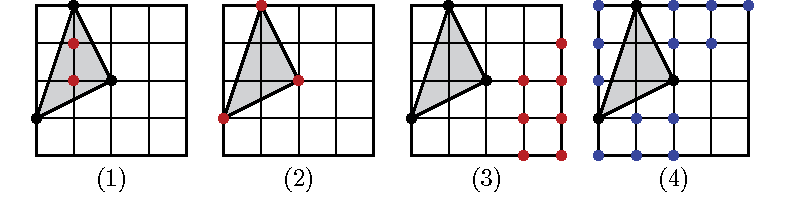
\includegraphics[scale=0.9]{boucle-mod}
    \caption{An illustration of the transition rule for a triangle (depicted in grey), depending on the placement of point $x$, colored red when the chain loops and blue when it does not loop: (1) $x$ belongs to $P\mathord{\setminus}\mathcal{V}$, (2) the convex hull of $\mathcal{V}\mathord{\setminus}\{x\}$ is $(d-1)$-dimensional, (3) $\mathcal{V}\cup\{x\}$ is not the vertex set of its convex hull, and (4) the transition changes $P$ into the convex hull of $\mathcal{V}\cup\{x\}$.}
    \label{fig:boucle}
  \end{center}
\end{figure}
\vspace{1ex}

By the above procedure, sampling a random lattice $(d,k)$-polytope consists in generating a random walk on the Markov chain until we are close enough to the stationary distribution. Thereby, the resulting random sampler for lattice $(d,k)$-polytopes is given by Algorithm~\ref{Algo.RS}.

\vspace{4ex}
\begin{algorithm}[H]\label{Algo.RS}
  \LinesNumbered
  \DontPrintSemicolon
  \KwIn{the dimension $d$, the size $k$ of the hypercube}
  \KwOut{a random lattice $(d,k)$-polytope}
  \BlankLine

  sample a random lattice $(d,k)$-simplex $P$ with vertex set $\mathcal{V}$\;
  \While{we are not close enough to the stationary distribution}{
  generate a random lattice point $x$ in $[0,k]^d$\;
  \If{$x \in \mathcal{V}$ and $\mathrm{conv}(\mathcal{V}\mathord{\setminus}\{x\})$ is $d$-dimensional}{
    $P \leftarrow \mathrm{conv}(\mathcal{V}\mathord{\setminus}\{x\})$\;
   }
  %\Else{$|\mathrm{conv}(\mathcal{V} \cup \{x\})|$ == $|\mathcal{V}| + 1$}{
  \Else{
    compute the convex hull $Q$ of $\mathcal{V}\cup\{x\}$\;
    \If{the vertex set of $Q$ is $\mathcal{V}\cup\{x\}$}{
      $P \leftarrow \mathrm{conv}(\mathcal{V} \cup \{ x\})$\;
    }
  }
 }
 \Return{$P$}
 \caption{Random sampling of a lattice $(d, k)$-polytope}
\end{algorithm}

\vspace{4ex}

In the other variant of our Markov chain, we introduce an additional rule when $P$ is a simplex: if the chosen random lattice point $x$ is a vertex of $P$, we may move that vertex to another lattice point instead of having a loop on $P$ in our Markov chain. More precisely, in this case we generate a new random lattice point $y$ in $[0,k]^d$ and compute the convex hull $Q$ of $[\mathcal{V}\mathord{\setminus}\{x\}]\cup\{y\}$. If $Q$ is $d$-dimensional, the transition goes from $P$ to $Q$, otherwise we loop on $P$. Note that, since $P$ is a simplex, $[\mathcal{V}\mathord{\setminus}\{x\}]\cup\{y\}$ is precisely the vertex set of $Q$ when $Q$ is $d$-dimensional. With this additional transition rule, we obtain Algorithm~\ref{Algo.RS2}.

\vspace{4ex}
\begin{algorithm}[H]\label{Algo.RS2}
  \LinesNumbered
  \DontPrintSemicolon
  \KwIn{the dimension $d$, the size $k$ of the hypercube}
  \KwOut{a random lattice $(d,k)$-polytope}
  \BlankLine

  sample a random lattice $(d,k)$-simplex $P$ with vertex set $\mathcal{V}$\;
  \While{we are not close enough to the stationary distribution}{
  generate random a lattice point $x$ in $[0,k]^d$\;
  \If{$x \in \mathcal{V}$}{
    \If{$|\mathcal{V}|=d+1$}{
      generate a random lattice point $y$ in $[0,k]^d$\;
      \If{$\mathrm{conv}([\mathcal{V}\mathord{\setminus}\{x\}]\cup\{y\})$ is $d$-dimensional}{
        $P\leftarrow\mathrm{conv}([\mathcal{V}\mathord{\setminus}\{x\}]\cup\{y\})$\;
      }
    }
    \ElseIf{$\mathrm{conv}(\mathcal{V}\mathord{\setminus}\{x\})$ is $d$-dimensional}{
      $P\leftarrow\mathrm{conv}(\mathcal{V}\mathord{\setminus}\{x\})$\;
    }
    %\If{$\mathrm{conv}(\mathcal{V}\mathord{\setminus}\{x\})$ is $d$-dimensional}{
      %$P\leftarrow \mathrm{conv}(\mathcal{V}\setminus\{x\})$\;
    %}
    %\Else{
      %generate random a lattice point $y$ in $[0,k]^d$\;
      %\If{$|\mathrm{conv}(\mathcal{V}\mathord{\setminus} \{x\} \cup \{y\})|$ == $d+1$}{
      %  $P\leftarrow \mathrm{conv}(\mathcal{V}\mathord{\setminus} \{x\} \cup \{y\})$\;
      %}
    }
   %}
  \Else{
    compute the convex hull $Q$ of $\mathcal{V}\cup\{x\}$\;
    \If{the vertex set of $Q$ is $\mathcal{V}\cup\{x\}$}{
      $P \leftarrow \mathrm{conv}(\mathcal{V} \cup \{ x\})$\;
    }
  }
 }
 \Return{$P$}
 \caption{Random sampling of a lattice $(d, k)$-polytope}
\end{algorithm}

\vspace{4ex}
%\vskip 12pt

The uniformity of both samplers is conditioned to the properties of the underlying Markov chains. These properties are studied in the next section.

\section{Properties of the Markov chain and uniformity of the sampler}\label{Sec.Pr}

It is well known that an irreducible, aperiodic, and symmetric Markov chain converges to the uniform distribution~\cite{levin2009markov}. In this section we prove that all these properties are satisfied by our Markov chains (reminders on their definitions will be given in the proof as well). Thus, we show that the two variants of our $d$-dimensional lattice $(d,k)$-polytopes sampler are uniform.

\begin{theorem}\label{Thm.MC}
  For all $d\geq2$ and for all positive $k$, the Markov chain corresponding to Algorithm 1 is irreductible, aperiodic and symmetric.
\end{theorem}

\begin{proof}
  Three properties have to be verified, thus this proof will be done in three steps. Let $P$ and $Q$ be in $\Omega$, and let $\mathcal{V}$ be the vertex set of $P$.

  \begin{enumerate}[i]
    \item \textit{Irreducibility.}
    A Markov chain is irreducible when all of its states can be reached from any other state. In other words the graph $\Gamma(d,k)$ underlying the Markov chain is connected. The vertex set of $\Gamma(d, k)$ is $\Omega$ and there is an edge in this graph between any two vertices that are related to one another by a single transition. The complete proof for the connectedness of $\Gamma(d,k)$ is quite involved and due to its length, we omit it here. This proof can be found in \cite{DavidPourninRakotonarivo2018}. An important piece of the proof consists in showing that, given a lattice $(d,k)$-simplex $S$, there always is at least one lattice point in $[0,k]^d$ that can be inserted as a new vertex in $S$. It turns out that proving this seemingly simple statement is quite tricky.

    \item \textit{Symmetry.}
    In order to prove the symmetry one needs to show that the probability $\mathbb{P}(P,Q)$ to move from $P$ to $Q$ in a single step is equal to the probability $\mathbb{P}(Q,P)$ of performing the opposite step.

    By our transition rules, for any $P \neq Q$ we have:

    $$
      \mathbb{P}(P,Q)=\mathbb{P}(Q,P) =
      \begin{cases}
        \frac{1}{(k+1)^d}, \text{ if }\exists x\in [0,k]^d \mbox{ s.t. } Q=
        \begin{cases}
          \mathrm{conv}(\mathcal{V}\mathord{\setminus}\{x\})\\
          \mathrm{conv}(\mathcal{V}\cup\{x\})
        \end{cases}\\
        0 \mbox{ otherwise.}\\
      \end{cases}
    $$

     \item \textit{Aperiodicity.}
     In order to prove that the chain is aperiodic, one needs to show that each state in $\Omega$ has period $1$. By definition, the period of a state $P$ is $\mathrm{gcd}(\mathcal{T}(P))$, where $\mathcal{T}(P)$ is the set of the return times in $P$. Since for an irreductible chain, all the states of $\Omega$ have the same period, then we need to find a state $P$ such that $\mathrm{gcd}(\mathcal{T}(P)) = 1$. Now recall that the polytope resulting from a transition in our Markov chain must remain $d$-dimensional. In particular, if one picks any vertex of a $d$-dimensional simplex $P$, this vertex cannot be removed, and we get a loop in our Markov chain. Since there exist $d$-dimensional lattice $(d,k)$-simplices for all $d\geq2$ and positive $k$, this shows that, at some state $P \in\Omega$ we have a positive probability to get back to $P$ from $P$ in one step.
     Hence, $1\in\mathcal{T}(P)$ and $\mathrm{gcd}(\mathcal{T}(P))$ is equal to~$1$.
   \end{enumerate}
\end{proof}

We now prove a similar result for our modified Markov chain.

\begin{theorem}\label{Thm.Move}
  For all $d\geq2$ and for all positive $k$, the Markov chain corresponding to Algorithm 2 is irreductible, aperiodic and symmetric.
\end{theorem}

\begin{proof}
  We proceed the same way as we did in the proof of Theorem~\ref{Thm.MC}.

  \begin{enumerate}[i]
    \item \textit{Irreducibility.}
    The proof still relies on the fact that one can always find a transition path between two simplices, yet the ``moving a vertex'' rule allows us to choose one vertex of the starting simplex and move it directly to a vertex of the desired simplex. Indeed, recall that by definition, a $d$-dimensional simplex is the convex hull of a set of $d+1$ affinely independent points. Therefore, one can transform any $P\in\Omega$ into a simplex by consecutive deletions of its vertices, until there only remains $d+1$ of them. With an analog reasoning, by a succession of addition of vertices, we always have a transition path from a simplex to a lattice $(d,k)$-polytope. The graph of the Markov chain remains connected, hence the Markov chain is irreducible.

    \item \textit{Symmetry.}
    Here the only difference from the symmetry proof in Theorem~\ref{Thm.MC} is that now we may have a one step transition between two simplices. It occurs when they only differ by a single vertex. Then, let $S$ and $S^\prime$ be two simplices in $\Omega$. If they only differ by a single vertex, then all the vertices of $S$ belong to $S^\prime$ apart from a vertex $x$, and all the vertices of $S^\prime$ belong to $S$ apart from a vertex $y$. The transition goes from $S$ to $S^\prime$ consists in choosing $x$, with a $\frac{1}{(k+1)^d}$ probability, and then to move it to $y$ with a $\frac{1}{(k+1)^d}$ probability. The same argument allows to treat the transition from $S’$ to $S$. Thus,
    $$
      \mathbb{P}(S,S^\prime)=\mathbb{P}(S^\prime,S)=
      \begin{cases}
        \displaystyle\frac{1}{(k+1)^{2d}} , \text{ if } S \text{ and } S^\prime \text{ differ by a single vertex,}\\
        0 \text{ otherwise.}
      \end{cases}
    $$

    \item \textit{Aperiodicity.}
    To prove the aperiodicity, it is necessary and sufficient to find a lattice $(d,k)$-polytope with a positive probability to loop. Let us consider a simplex $S$ with vertex set $\mathcal{V}$ and a lattice point $x \in [0,k]^d$. If $x$ is chosen among the vertices of $S$, then we have to redraw a point $y\in [0,k]^d$ where we decide to move $x$. The cases when we have a loop on $S$ are: either $y$ and $x$ are the same point, or $\mathrm{conv}([\mathcal{V}\mathord{\setminus}\{x\}]\cup\{y\})$ is not a $d$-simplex. Note that the probability to choose $x$ again is $\frac{1}{(k+1)^d}$.
    Therefore,
    $$
      \mathbb{P}(S,S)\geq{\frac{d+1}{(k+1)^d}\cdot\frac{1}{(k+1)^d}}>0.
    $$
    Thereby, $S$ has period $1$. Since the chain is irreducible, each state of $\Omega$ has the same period $1$. Hence, the chain remains aperiodic.
  \end{enumerate}
\end{proof}

It is an immediate consequence of Theorem~\ref{Thm.MC} and of Theorem~\ref{Thm.Move} that the two variations of our Markov chain have a uniform stationary distribution. Thus, the lattice $(d,k)$-polytopes obtained from both samplers are picked uniformly from $\Omega$. We have the following theorem.

\begin{theorem}\label{Thm.RS}
  The random samplers described in Algorithm~\ref{Algo.RS} and in Algorithm~\ref{Algo.RS2} are uniform random samplers for $d$-dimensional lattice $(d,k)$-polytopes.
\end{theorem}

\section{A lower bound on the mixing time}\label{Sec.Mix}

Recall that the total variation distance is a distance measure between probability distributions~\cite{levin2009markov}.
The effectiveness of the sampler is given by the number of steps it takes until one is close enough to the stationary distribution on $\Omega$, meaning that the total variation distance between the current distribution
and the stationary one is less than a small positive quantity $\varepsilon$. This number of steps is called the mixing time of the Markov chain, denoted $t_{mix}(\varepsilon)$. That is, the quicker the Markov chain mixes, the more effective the resulting sampler is. Obtaining an accurate estimation of the mixing time is often a difficult problem. In order to obtain a lower bound, one may use the diameter of the graph of the Markov chain. This diameter is the length of the longest geodesic walk on the chain between any two states.
In our case, that length is bounded below by the difference between the largest number of vertices of a $d$-dimensional lattice $(d,k)$-polytope and the number of vertices of a $d$-dimensional simplex.

The largest number of vertices of a lattice polygon contained in a disk or a square has been studied in~\cite{AcketaZunic1995,T91,BB91}. Deza, Manoussakis and Onn have generalized this result to higher dimensions by describing lattice $(d,k)$-polytopes whose diameter is large and conjecturally maximal~\cite{DezaManoussakisOnn2018}. According to~\cite{AcketaZunic1995}, the largest number of vertices of a lattice polygon contained in $[0,k]^2$ is

\begin{equation}\label{Eqn.Deza}
  12\left(\frac{k}{2\pi}\right)^{2/3}+O(k^{1/3}\log{k})\mbox{.}
\end{equation}

We therefore immediately obtain the following lower bound on the mixing time of our sampler in the $2$-dimensional case from equation (7.3) in~\cite{levin2009markov}.

\begin{theorem}\label{Thm.Lowerbound}
Assume that $d=2$. For any $\varepsilon>0$, there exists $c>0$ such that
$$
t_{mix}(\varepsilon)\geq{ck^{2/3}}\mbox{.}
$$
\end{theorem}

For the case of higher dimensions,  B{\'a}r{\'a}ny and Larman gave bounds on the number of faces of each dimension of a lattice polytope contained in the the $d$-dimensional ball of radius $r$ centered at the origin as a function of $r$ and $d$ \cite{barany1998convex}. In particular they provide bounds on its number of vertices. Up to a translation and finding the right constant, Theorem 1 in~\cite{barany1998convex} also provide us the following lower bound on the mixing time.

\begin{theorem}
  For any $d\geq 2$ and for any $\varepsilon>0$, there exists $c>0$ such that
  $$
  t_{mix}(\varepsilon)\geq ck^{d \frac{d-1}{d+1}}\mbox{.}
  $$
\end{theorem}

We have carried out a number of experiments in order to get an estimation of the actual mixing time of the sampler corresponding to Algorithm~\ref{Algo.RS} in the $2$-dimensional case. These results are presented in Section~\ref{Sec.Res}.

\section{Experimental results}\label{Sec.Res}

The empirical estimations we obtained are based on ergodic theory.
% average number of vertices
\noindent
\begin{figure}[b!]
  \begin{center}
  %\hspace{-1cm}
    \begin{minipage}[c]{.49\linewidth}
      \includegraphics[scale=.20]{averageVertices}
    \end{minipage}
    \begin{minipage}[c]{.49\linewidth}
      \includegraphics[scale=.20]{averageVolume10M}
    \end{minipage}
    \caption{The average number of vertices over a same long run after $100$ thousand, $1$ million, and $10$ million steps is shown on the left when the size $k$ of the box satisfies $2\leq k<100$, together with the theoretical maximal diameter of a lattice polygon contained in $[0,k]^2$, that is half of the quantity~(\ref{Eqn.Deza}). The average area of the visited polygons over a $10$ millions steps is shown on the right.
    \label{Fig.NV}}
  \end{center}
\end{figure}
This theory requires the studied Markov chains to be irreducible and positive recurrent. These properties hold in our case since we have a finite space of states~\cite{levin2009markov}. Ergodic theory states that the average of any real-valued function on the states over a long enough walk is the same as the expectancy at the stationary distribution, see Theorem 4.16 in~\cite{levin2009markov}. Here the function can be any quantity we can measure on lattice $(d,k)$-polytopes. The process is the following: we run a long walk on the Markov chain, evaluate the quantity on each state we visit, then calculate the average value of this quantity over the whole run.
Our results are reported in Figure~\ref{Fig.NV}. One can see that the average number of vertices of a polygon seems to stabilize after $100$ thousand steps (resp. $1$ million and $10$ million) when $k\leq 20$ (resp. $k\leq 30$ and $k\leq 50$).
We also measured the average area of a polygon after a $10$ million steps walk and show it on the right of the same figure. Our measures suggest that
$$
\mathbb{E}[n] \ge 6\left(\frac{k}{2\pi}\right)^{2/3} \text{ and } \mathbb{E}[a] \leq \frac{3}{4} k^2,
$$
where $\mathbb{E}[n]$ and $\mathbb{E}[a]$ are respectively the expectancy of the number of vertices and the area of a polygon at the stationary distribution.

The coupling method is another way to estimate the mixing time. The coupling is more general and often used to bound rates of convergence to stationarity as well. It consists in running two walks on the Markov chain.
The coupling result on Markov chains tells us that once two coupled walks are at the same state, they will both move following the stationary distribution with high probability. Note that the walk may have been already very close to the stationary distribution much earlier.
Our computations allowed us to get an empirical upper bound on the  mixing time in the $2$-dimensional case for $k$ up to $6$, the computation time becoming prohibitive for larger values of $k$.
Table~\ref{Tab.Coupling} presents execution times for this method and the number of steps needed for the two walks to meet.
As one can see, the required number of steps increases quickly. This suggests that the coupling method may not provide sharp estimations of the mixing time for our sampler.

\begin{table}[t!]
  \centering
  \caption{Time needed to reach the stationary distribution with two coupled walks. The first walk is starting at the corner simplex with vertices $(0,0)$, $(1,0)$, and $(0,1)$. The second walk is starting at the opposite corner simplex with vertices $(k,k-1)$, $(k-1,k)$, and $(k,k)$.}
  \label{Tab.Coupling}

  \bigskip

  \begin{tabular}{|c|r|r|}
    \hline
    $k$ & Number of steps & Execution time\\
    \hline
    1 & 2 & 0.001s \\
    2 & 5026 & 0.164s \\
    3 & 42247 & 1.368s \\
    4 & 11387661 & 6m11s \\
    5 & 78745909 & 42m45s \\
    6 & $3.928 \times 10^9$ & 2133m20s \\
    \hline
  \end{tabular}
\end{table}

\bibliographystyle{alpha}
\bibliography{biblio.bib}

\end{document}
